% Mit twoside als weitere Option werden die Seitenränder angepasst, sodass beidseitig gedruckt werden kann
\documentclass[pdftex,12pt,a4paper]{report}

\usepackage[]{dbstmpl}
%\usepackage[english]{babel}
\usepackage{graphicx}
\usepackage{hyperref}
\usepackage{microtype}
%\usepackage{subfig}
\usepackage{amsmath}

\usepackage{tikz}
\usetikzlibrary{matrix,chains,positioning,decorations.pathreplacing,arrows}
\usepackage{forest}
\usepackage{subfigure}

\usepackage{pgfplots}
\pgfplotsset{compat=1.8}
\usepackage{layout}
%\usepackage{showframe}
%\usepackage{geometry}

%Simons latex code start
\usepackage{listings}
%\usepackage{microtype}


\lstset
{
    basicstyle=\ttfamily\scriptsize,
    numbers=left,
    stepnumber=1,
    showstringspaces=false,
    tabsize=1,
    breaklines=true,
    frame=TLrb,
    breakatwhitespace=false,
}
\renewcommand{\thesubsection}{\alph{subsection})}
\renewcommand{\labelitemi}{$-$}
\newcommand{\inlinecode}[2]{\lstinline[language=#1]$#2$}
%\fxusetheme{color}
%Simons latex code end

\global\arbeit{Master Thesis}
%\global\arbeit{Masterarbeit}
%\global\arbeit{Seminararbeit}


% Hier die eigenen Daten eintragen
\global\titel{Explainable Artificial Intelligence by Expanding Expert Solutions with Genetic Programming}
\global\bearbeiter{Simon Fehrer}
\global\betreuer{Dr. Michel Tokic, Dr. Steffen Udluft, Dr. Daniel Hein}
\global\aufgabensteller{Prof. Volker Tresp}
\global\abgabetermin{29.02.2019}
\global\ort{Munich}
\global\fach{Computer Science}

\begin{document}
\deckblatt

\erklaerung

\begin{abstract}
Abstract will soon be updates meh
Machine-learning offers great potential for finding high performance solutions in plenty of areas.  However, the more delicate an environment gets, the higher is the reserve to use ``blackbox'' solutions, which can make momentous decisions. We propose a new approach, which addresses this problem by improving heuristics with genetic programming that creates easily understandable policies.

\end{abstract}

% Inhaltsverzeichnis (abhaengig von der Laenge des Dokuments)
\tableofcontents

% Hier beginnt der Hauptteil

%\chapter{Introduction}

In this thesis, a novel approach for explaining black box machine learning solutions is proposed and evaluated.

The current state of the art in artificial intelligence (AI) is mostly based on the use of complex data structures such as neural networks. Although their performance is beyond question, they must nevertheless be considered as black boxes due to their scope and complexity, which means that humans lose the ability to control and understand decisions made by machines.

Originating from an explainable solution provided by an expert, genetic programming (gp) is used to generate improved solutions which perform like neural network while being as explainable to the expert as possible.
Several techniques were implemented to improve explainability. This includes the use of a distance measurement to the experts program, genetic evolve operators that are strongly linked to the original program, having the opportunity to leave a core of the origin untouched and many more.

The Pareto efficient candidates, which always represent the greatest improvement to a given complexity increase, can ultimately be weighed on the basis of explainability and fitness. If the expert already had the wrong approach, it can be uncovered and thus reveal core problems in the solution.

To verify the approach, many versions of the approach were tested. As a benchmark, well-known reinforcement learning environments such as the gym mountain car and cart pole were chosen, as well as the industrial benchmark to test more complex controllers in sensitive environments.
%\chapter{Related work}

\section{TODO2 Motivation} 
Although artificial intelligence has been a household name since the 1950s \cite{Rosenblatt58theperceptron:}, it has been experiencing a new boom for some years now, the end of which is not yet in sight.
The main reason for the ongoing high interest is the continuously increasing number of cases where machine learning (ml) outperforms man many times over, even with relatively low cost.
This could be achieved by the ever-increasing computing power, which together with the continuing achievements in research, all of a sudden, made things possible that were considered unsolvable some decades ago.
An example of this event is deep blue, a chess computer which in 1996 was able to beat the then world champion in chess, Garry Kasparov. What was a revolution at that time is rather unimpressive today, because everyone who owns a mobile phone with a chess app has a much more powerful tool in his pocket. [todo source, ich mach hier kein schach?]

Today, not only are far more complex problems being solved , ki is also becoming more and more prevalent in everyday life. [genes, alpha go][todo, speech recognition, word spelling, other assists, smart home, recommendations].

\section{Machine learning with neural networks}


\subsection{Supervised learning}

Supervised learning [todo image] is the task of learning a function that, for any given data, maps inputs to outputs only by training on samples of known data. This is mostly done by using neural networks which derive a mapping from the inputs to outputs. An example is labeling animals on image inputs correctly or recognizing handwritten letters.  [todo cite?]  

\subsection{Reinforcement learning}
Reinforcement learning [todo image] features an agent which has the task of learning the optimal behaviour in an environment without any default knowledge. To do so, the agent receives a reward for actions it performed as well as the state of the environment that it is currently in. In order to choose the best action, the agent has to learn a policy for all possible states. To improve the policy, the agent both has to exploit the experience that was made in the past, but also has to explore new possible solutions. This is called the exploration-exploitation tradeoff. [todo cite]

The problem is similar to supervised learning as a mapping from inputs to outputs has to be learned with the main difference being that no ``right'' decisions are known.
Well known examples are bots playing computer games like pong, doom or chess. [todo cite][todo images] For a long time, reinforcement learning was limited to rather simple, discrete problems. When state spaces are very large, for example in chess or in games with multi-dimensional continuous state spaces like 3d games have to be approximated. An option to do so is tiling [todo cite], but the major breakthroughs were achieved by using neural networks aswell. In reinforcement learning, they can be used to perform exactly this mapping.

\subsection{Neural networks}

\cite{Rosenblatt58theperceptron:} 
In order to find out whether and how one can resolve the logic within a neural network, we have to take a closer look at the functionalities.

Artificial neural networks are computing systems inspired by the biological brain. Such systems ``learn'' to perform tasks by considering examples, generally without being programmed with task-specific rules. The brain is made up of neurons which can activate each other to lead to a decision.

An artificial neural network is modeled with artificial neurons that are strung together in form of layers. The layers are connected in series between the neurons can communicate with each other. To calculate its own activation, a neuron receives signals from neurons in the proceeding layer. Every incoming signal gets multiplied with a specific weight which then is summed up and put into an activation function. The resulting activation is then sent to a set of neurons in the next layer. If the resulting output is correct, the weights can stay the same. If it is wrong though, the error is fed back through all layers with an algorithm called backpropagation where the weights are adjusted to support making the right decision next time.

\input{tikz/neural_networks/neural_network_layers}

\begin{figure}
    \centering
    \input{tikz/neural_networks/artificial_neuron}
    \caption{Artificial neuron with three input values}
    \label{tikz artificial neuron}
\end{figure}

Popular activation functions are the sigmoid function:
${sig}(t) = \frac{1}{1 + e^{-t}}$
aswell as the rectified linear unit function (ReLu):
$f(x)=\max(0,x)$

\begin{figure}
    \centering
    %\hrulefill
    %\fbox{
        \begin{minipage}[t]{0.40\textwidth}
        \input{tikz/neural_networks/graph_relu}
        \end{minipage}
        %}
    \hspace{5mm}
    %\fbox{
        \begin{minipage}[t]{0.40\textwidth}
        \documentclass{standalone} %[varwidth=\maxdimen,convert,border=5pt]
\usepackage{pgfplots}
\usepackage{tikz}
\usepackage{amsmath}
\begin{document}

\centering
\resizebox{\columnwidth}{!}{
    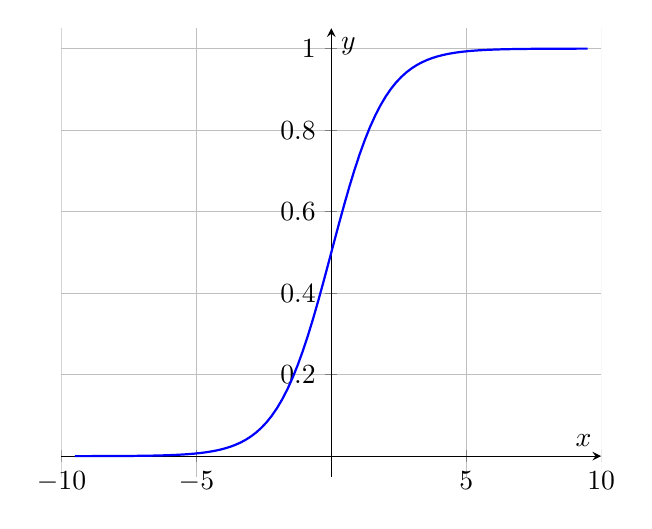
\begin{tikzpicture}
    \begin{axis}[
        grid=major,
        axis lines=middle,
        xmax=10,
        xmin=-10,
        ymin=-0.05,
        ymax=1.05,
        xlabel={$x$},
        ylabel={$y$}
    ]
    \addplot [domain=-9.5:9.5, samples=100, thick, blue] {1/(1+exp(-x)};
    \end{axis}
    \end{tikzpicture}
}

\end{document}
        \end{minipage}
    %}
\end{figure}


Artificial neural networks are computer systems that are strongly oriented towards the biological brain. An input vector is received by neurons, which in turn can activate other neurons. At the end of this process there are some neurons that can control an action.
In royal neural networks this principle is abstracted in layers of neurons. An input layer receives all important information and an output layer evaluates all possible actions - the best one is then taken. Between the two layers there can be any number of hidden layers. Their task is to divide the problem between the input layer and the output layer and to identify subproblems. The training process will be started with a random parameterization and the decisions will be very bad at the beginning. If a wrong decision is made, the neurons from output to input adjust their values so that the next time the right decision is made.

A neuron is modeled as follows (see Neuron). For a group of neurons from the previous layer (often all neurons) the signals are received and weighted. Together with a bias, which is added by the neuron itself, a sum is formed. To prevent unnaturally large values in neurons, the sum is added to an activation function that calculates the final activation of the neuron. Common activation functions include ReLu and Sigmoid. The result is then passed on to the neurons of the next layer.

The complexity of such a network depends on the number of layers, the number of nodes per layer and the type of interconnection between layers.
A possible network to solve Mountain Car could be for example an input layer with two neurons and an output layer with three neurons, as well as three hidden layers with 24, 48 and 24 layers each. Full connectivity between the layers is not unusual, resulting in the following number of connections:

 $2 \cdot {input} \cdot 24 \cdot 48 \cdot 24 \cdot 3 {output} = 165888$
 [todo formeln einfügen?]
the system thus consists of n $165888$ variables.

There is one thing that is decisive for the explainability: no matter at what point in time the network is viewed, it always has the same complexity. The only way to get better is to adjust the values within the given complexity.
connections (excluding $w_0$) and 101 neurons. [https://towardsdatascience.com/reinforcement-learning-w-keras-openai-dqns-1eed3a5338c] 

Over the years, many architectures of neural networks have been developed, which can often solve a specific problem very well. Worth mentioning are [todo, such as: convolutional neural networks, lstm, autoencoder, numerous activation functions, mcts, dqn double dqn, rainbow, ... Soll ich ein paar erwähnen?]. \cite{AIINDEX2019} 

[todo, wie genau Seitenzahl zitieren bei häufigerer Zitierung?]

\section{ML failure examples}

The continuing trend in the field of artificial intelligence also harbours some inconvenience.

In 2018, the Tesla autopilot caused a fatal accident because it mistook a truck standing crossways for a road sign. In 2015, one company caused a stir by claiming to have played a major role in the presidential election in America and the Brexit decision in Great Britain by means of data mining. Elon Musk and Stephen Hawking have both explicitly warned about the risks of artificial intelligence.
Apart from these horror scenarios, there are other reasons why it is not easy to dispense with the explanations.

\begin{itemize}
    \item How can false decisions be solved? Debugging and correcting false decisions by hand is almost not possible. How do I find out why a wrong decision was made? How can I change the behaviour without making mistakes in other places?
    \item How can you guarantee behaviour?
    \item How can you integrate small changes to the requirements of a neural network without new training processes?
    \item How can I apply this approach in a delicate environment?
    \item How to convince another person of my solution?
    \item How to justify in court a wrong decision of a machine?
    \item Even small changes in demand lead to a new training process
    \item Non-experts do not feel confident using the solution [todo zitat]. Rumours of machines learning to be evil [TODO rewrite] are widespread [TODO Zitat].
\end{itemize}

\subsection{Explaining how neural networks make decision}

Neural networks are insanely complex at all times. The attempt to gain information by analysing the values of neurons is therefore doomed to failure from the outset. Nevertheless, there are ways to extract information from the network. One possibility, is to look at the decisions and try to identify a structure behind them. It is also possible to look at parts of the neural network in isolation in order to deduce their function.

\subsection{Trusting a neural network}


Machine learning approaches can not be verified, the reliability can not be ``guaranteed''. Even more, they knowingly perform very poorly during the start of the training process. The trust into the reliability solely comes from its outstanding performance. A neural network will only be accepted as solution when the fail rate is so low that it is statistically insignificant. 

\subsection{Sensitive environments}

Companies that work with sensitive environments are particularly interested in preserving the explainability. We are certainly still a long way from having a nuclear power plant controlled by a neural network, but there are many areas where a controller makes decisions for a system where, in addition to many very good decisions, one single, wrong decision can lead to very great damage, for example to a gas turbine.
environments like these make it impossible for an agent to explore, so RL cannot be used or only with great restrictions.





\section{What is considered explainable?}

There are neural networks from which humans can extract information extremely easily: Our own brain. It is not only the most complex structure in the universe, it is also more energy-efficient than all artificial versions and, moreover, it already has a lot of instinct and life experience. physics applies everywhere to the same extent, which is why solutions found in certain areas can often be transferred to others in a similar form. [todo cite, idea] developers and experts have the wonderful ability to extract this information so efficiently that they can formulate a heuristic as a program after a short training period, often without any training at all.

Programs are probably the simplest way to describe a complex function.

Good coding style is a virtue even among experienced developers. In order to be able to understand programs written by computers as far as possible, special quality criteria apply. For our approach we have introduced some original features to achieve this.

%\input{texfiles/03_Approach}
%\chapter{Experiments}
This chapter presents the benchmarks against which the approach has been tested. This includes mountain car (MC) and cartpole (CP), as well as the Industrial Benchmark (IB). The first benchmarks are widely used, simple toy benchmarks, where the concept can be tested well. The IB is, in contrast, a stochastically independent, high-dimensional testbed, which was especially designed for the simulation of very complex processes in industry for reinforcement learning.

% todo regression aswell?



 \section{Industrial benchmark}
 
The Industrial benchmark was introduced by scientists at Siemens to meet the high requirements of complex industrial processes. \cite{industrialBenchmark}
 
 

\section{Mountain car}\label{experiment:mountaincar}

With the Mountain car problem, a car is supposed to drive up a mountain that is too steep for the car's engine. To achieve is to build up momentum to reach the target as fast as possible given the position $p$ and velocity $v$ of the car.

% todo hein "o-dimensional state space s = (r, ˙r)"

\begin{figure}[ht]
	\centering
  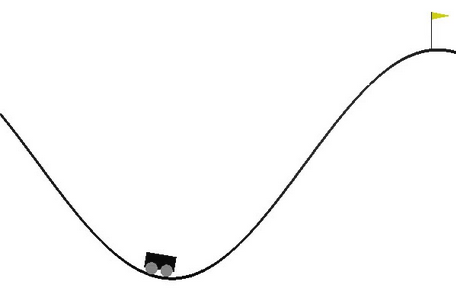
\includegraphics[scale=0.6]{img/MTC/MTC_experiment.PNG}
	\caption{A possible starting position in MC}
	\label{img:mtc_experiment}
\end{figure}

In the discrete version of MC there are three possible actions:

\begin{tabular}{ll}
\hline 
Num & Action\tabularnewline
\hline 
0 & push left\tabularnewline
1 & no push\tabularnewline
2 & push right\tabularnewline
\hline 
\end{tabular}

The problem was first introduced in 1990 \cite{mountaincarOriginal} and has since become a widely used RL benchmark.

\begin{tabular}{|c|c|c|c|}
\hline 
Num & Observarion & Min & Max\tabularnewline
\hline 
\hline 
0 & position & -1.2 & 0.06\tabularnewline
\hline 
1 & velocity & -0.07 & 0.07\tabularnewline
\hline 
\end{tabular}

\begin{tabular}{|c|c|}
\hline 
Num & Action\tabularnewline
\hline 
\hline 
0 & push left\tabularnewline
\hline 
1 & no push\tabularnewline
\hline 
2 & push right\tabularnewline
\hline 
\end{tabular}






\subsection{Learning goals on the way to the perfect solution }

Attempts to reduce the distance to the target by accelerating in its direction are quickly recognized as unsuccessful. 
In order to reach the target at all, the agent must learn to gain momentum with the help of the counter slope. This can be achieved, for example, with the "simple" heuristic of always accelerating in the direction in which one is currently moving.

This way you always reach your goal, but there is still plenty of room for optimization.
These are:
\begin{itemize}
\item Turn back early: To reach the goal, you don't have to take the maximum momentum. If you turn back earlier, a lot of time can be saved.
\item Discard Action 1 "Do nothing": Doing nothing makes no sense in principle - speed is lost when taking a swing and when turning around, instead of doing nothing two consecutive times, you could normally accelerate in the opposite direction.
\item Number of necessary swings: Depending on starting position of experiment, target can be reached by two or three starts. The agent must therefore decide in the initial state already in which direction to start. A safety buffer does not have to be taken into account, since all other states are deterministic.
\end{itemize}

\paragraph{Problems}

The initial state is a major problem for regression analyses because, despite its crucial role, it occurs only once in the data set. For this reason, there are sometimes large differences in performance when testing the agents.
Just past is also beside the point. Some Sarsa runs end with very tight finishes. Some runs of the trained agents are unfortunately not lucky and have to turn back shortly before the finish.

The SARSA approach was chosen because it was the fastest that could solve mountain car well. However, this meant that little was explored in the learning process and often there are wrong decisions that 
   but there's still a lot of air up there. Very easy to learn that the goal can be achieved with less momentum and you can turn with 

funfact:
cartvel < 0 then 0 else 2
cartvel <= 0 then 0 else 2 

Reverse early

This simple policy can further be improved, where the most efficient way is probably by reversing early on the opposite side. 

\paragraph{Close-form preset policy}

In \cite{xiao2019}, a close-form preset policy was proposed, defining a lower and upper bound  for the car to determine the actions.
\begin{figure}
    \centering
    
    \begin{lstlisting}
    push right, when:\\
    $min(-0.09(position + 0.25)^2+0.03, 0.3(position + 0.09)^4-0.008)\\
    \leq velocity \leq \\
    (-0.07(position + 0.38)^2 + 0.07)$\\
    push left instead
    \end{lstlisting}
    \caption{Pseudocode for getting first layer of modifiable nodes}
    \label{code:MC-agent:preset_policy}
\end{figure}

\paragraph{Real solution, optimal solution and expert abstraction}

As we will see and discuss in \ref{todo}, the first decision is most relevant for the optimal solution. The starting velocity is always 0, but depending on the starting position, you have to take three or four turns to reach the goal. For this purpose, another expert policy has been implemented, which explicitly emphasizes this state.


\subsection{Machine learning approach}

    
\begin{figure}[ht]
	\centering
  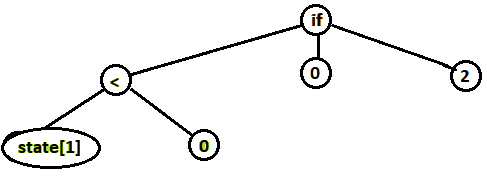
\includegraphics[scale=0.6]{img/MTC/mtc_simple_tree.png}
	\caption{Computational tree of the simplest program}
	\label{img:mtc_simple_tree}
\end{figure}

The only real requirement of the approach is that it performs better on average than the explainable approach and is based on a neural network. Conveniently, the gym-environment has a leaderboard containing the approaches that have been able to learn the fastest to create a policy that solves the problem in steps of less than $110$. \ref{mtc_leaderboards}
The approach chosen here is a SARSA procedure [TODO paper Sarsa? Approach?] with tiling that is able to learn a sufficient policy after 75 episodes with an average episode reward of $\approx-103.4$.

The same approach war also trained for 200 episodes but a better average result of $\approx-98.7$

\begin{tabular}{l l l}
  Agent   & Training episodes  & Average episode reward (100 runs) \\\hline
  Sarsa 75 &  75  &  -103.41 \tabularnewline
  Sarsa 200 &  200  &  -98.68 \tabularnewline
  Sarsa 1000 &  1000  &  -106.78 \tabularnewline
  Sarsa 10.000 &  10000  &  -109.31 \tabularnewline \hline
  Simple agent & ($<$) & -119.41 \tabularnewline
  Bad simple agent & ($<=$) & -129.62 \tabularnewline \hline
  Fix preset Policy & & -102.61 \tabularnewline
  
\end{tabular}


\noindent For this initial experiment, the black box is explicitly not , the way it works was deliberately not looked at in detail.

\paragraph{First evaluation} 

The ``simple'' policy reached the target with an average episode reward of $-119$ without fails very constantly. The average reward of the SARSA-agent is, with an average reward of $103$, outperforming the ``simple'' approach with about $14\%$.
A grain of salt however is, that the SARSA Approach seems to be relatively unstable, even causing the policy to almost fail to reach the target in 200 steps, as can be seen in \ref{img:MTC-heuristic-vs-sarsa-reward}. The reason for poor performance was not evaluated, even though it can be assumed that this is caused by uncommon starting states where not enough experience was made yet. [todo epsilon wert = 0?] 


\begin{figure}[ht]
	\centering
  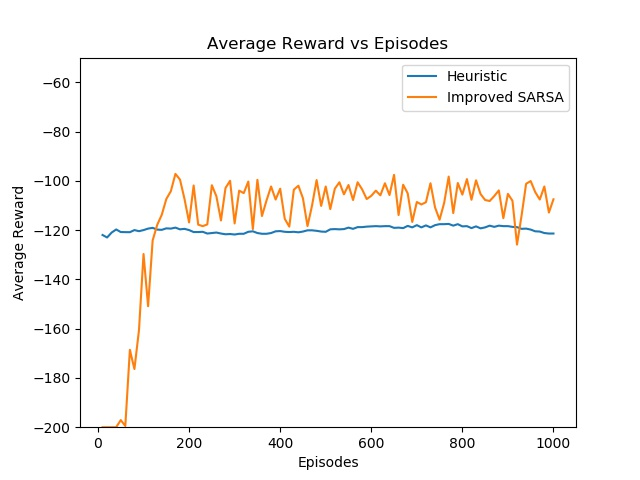
\includegraphics[scale=0.4]{img/MTC/MTC-heuristic_vs_sarsa-1000-10-average.jpg}
  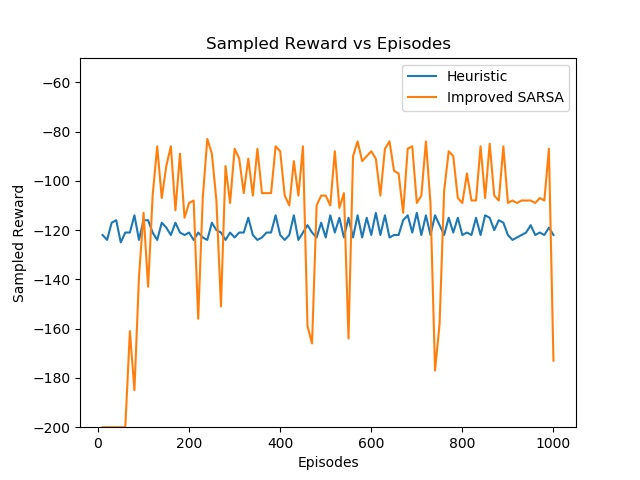
\includegraphics[scale=0.4]{img/MTC/MTC-heuristic_vs_sarsa-1000-10.jpg}
	\caption{SARSA implementation learns to outperform the heuristic on average}
	\label{img:MTC-heuristic-vs-sarsa-reward}
\end{figure}


    % TODO. Zeigen, wie RL nach einer Zeit besser als die Heuristik abschneidet
    % TODO: RL machen auch manchmal doofe Sachen. Zappeln im Reward, beispielsweise


    


\subsection{GP preparation}
The samples sample size of the data resulted from going through 15 complete runs of mountain car with the chosen SARSA-Approach. These runs were taken randomly and all observations and decisions were considered, resulting in about $2000$ samples. The data was then split into 80\% training and 20\% test data to verify the results.\\




\subsection{Missing action ``no push''}

Action ``no push'', even though it is possible, 

One aspect of ignoring all information from the black box was to create a mountain car core solution that does not allow it to stand still whereas the black box solution considered option '0' of not moving. This option was used in $134/2088$ samples, which is about $6.4\%$\\

[todo insert picture of the tree and/or the sarsa choices]\\
This is already a relatively large, categorical difference to the expert, which raises many questions.
Has this limitation perhaps already caused a gross error? Is the gp process affected by this?
This question is indeed difficult to answer. Action ``no push'' is in fact hardly relevant for solving the problem, since a quick turn around by reversing the acceleration is more efficient than doing nothing. This limitation is in fact an area of core logic of the expert program that precedes the SARSA approach. However, if this decision has not been made as the conclusion of an analysis, action ``no push'' may need to be reconsidered.
Thus, while this restriction is legitimate from a logical point of view, from a technical point of view it also causes problems in regression. Not only can the cases not be matched, because all actions are equally wrong, these data points have no influence and could be ignored. Considering that exactly these reversal areas are of great relevance, it is questionable how much this affects the result.

In order to explore the effects, an equivalent program was written, which could additionally select the option ``no push''.

Main differences: 
- lower regression error
- No fitness improvement
- Less variance
- More effort at the GP
- more complex trees



\begin{figure}
    \centering
    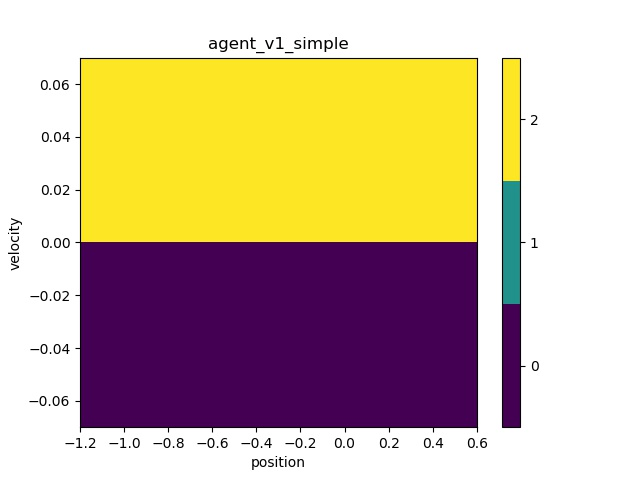
\includegraphics[width=.4\linewidth]{img/MTC/decision_plots/agent_v1_simple.jpg}
    \caption{A subfigure}
    \label{fig:subf1}
\end{figure}
\begin{figure}
    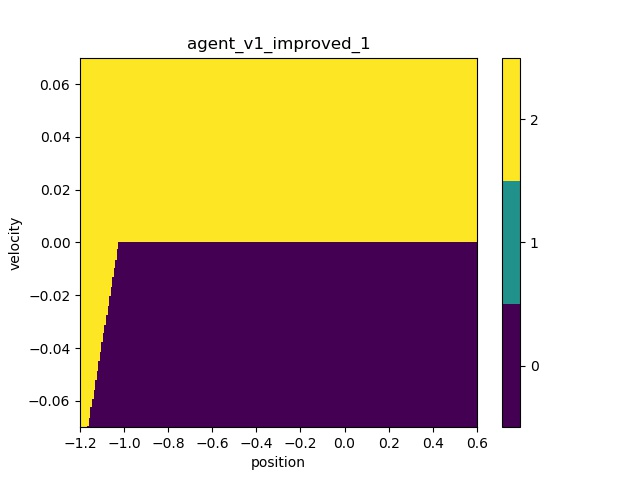
\includegraphics[width=.4\linewidth]{img/MTC/decision_plots/agent_v1_improved_1.jpg}
    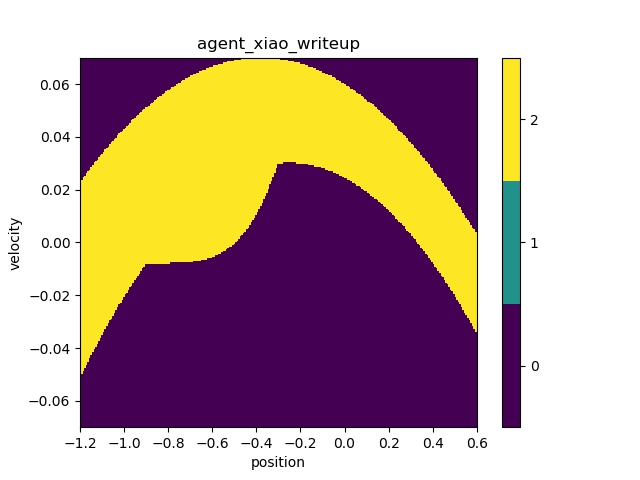
\includegraphics[width=.4\linewidth]{img/MTC/decision_plots/agent_xiao_writeup.jpg}
    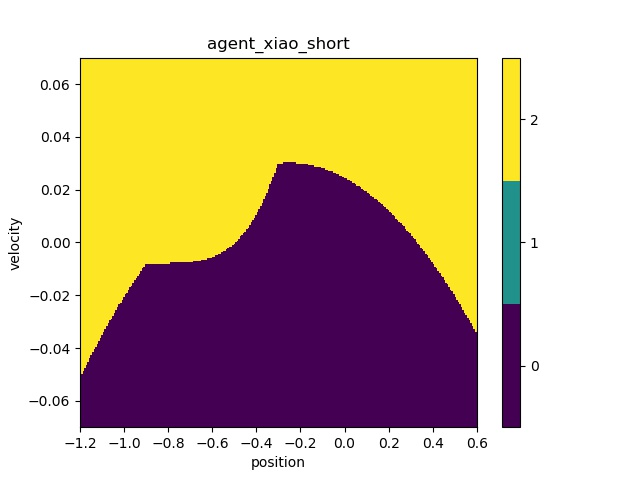
\includegraphics[width=.4\linewidth]{img/MTC/decision_plots/agent_xiao_short.jpg}
\end{figure}
\begin{figure}
    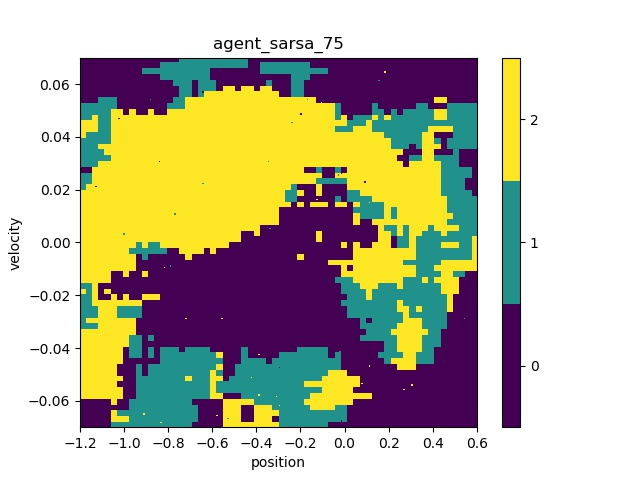
\includegraphics[width=.4\linewidth]{img/MTC/decision_plots/agent_sarsa_75.jpg}
    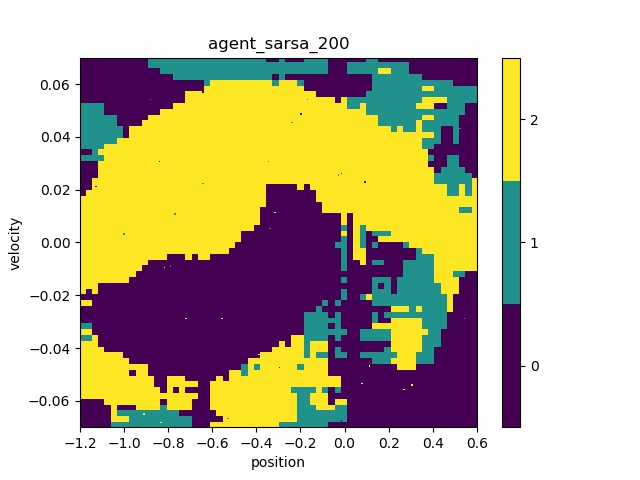
\includegraphics[width=.4\linewidth]{img/MTC/decision_plots/agent_sarsa_200.jpg}
    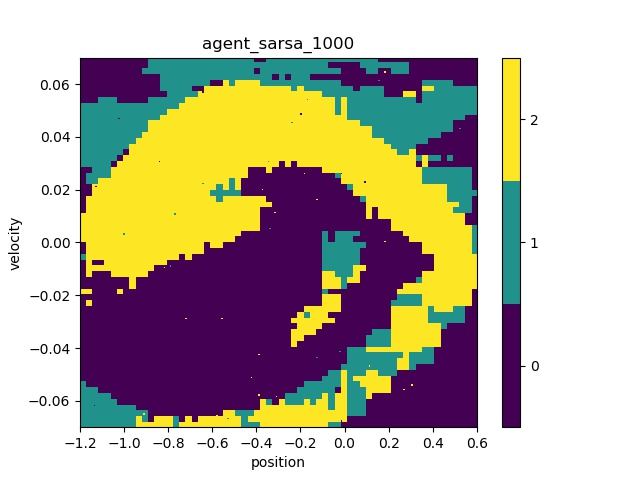
\includegraphics[width=.4\linewidth]{img/MTC/decision_plots/agent_sarsa_1000.jpg}
    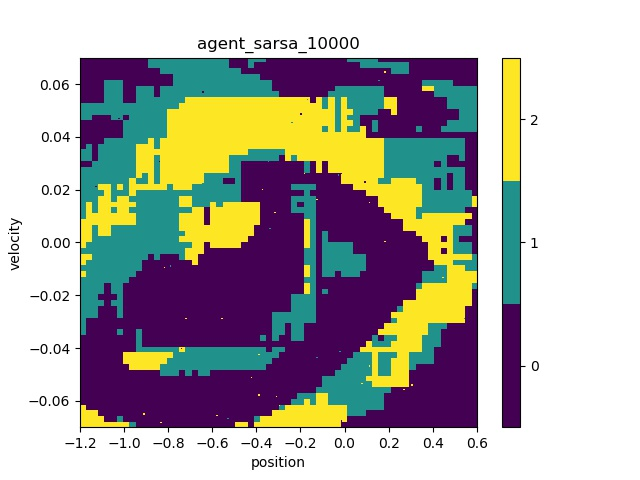
\includegraphics[width=.4\linewidth]{img/MTC/decision_plots/agent_sarsa_10000.jpg}
    \caption{Caption}
    \label{fig:my_label}
\end{figure}


\subsection{Reference programs}

The genetic improvement process was applied to numerous reference programs of which the following were thoroughly evaluated.

\begin{itemize}
    \item simple policy: ``Move towards the moving direction''
    \item simple fix: the simple policy with the decision for either 0 or 2 is not changeable by the genetic programming process
    \item simple fix extended: the simple policy with another if statement allowing to perform action ``no push'' aswell
    \item little expert: simple agent reversing earlier on the last turn
    \item true expert: compact but high end program that exceeds the fitness of sarsa75 
    \item closed policy: current lederboard leader
\end{itemize}


\subsection{fitness kernel fitting error regression [todo what name?]}

Mountain car's action space ${0, 1, 2}$ is ordered and scaled. The performance can therefore be calculated with some sort of regression kernel instead of only fitting result matches.

The action space further is one discrete dimension, leaving plenty of options to unitize the evaluation process:

\begin{itemize}
    \item one-hot encoding.
    
    All actions are one-hot encoded for which a softmax-probability is calculated [TODO softmax]. This does resemble the structure of a regular program though, what makes it difficult to use the tree edit distance.
    
    \item Return the action as part of the gp-process evaluation. If a value is not discrete, a value must be assigned.
\end{itemize}

The following regression kernels were evaluated for their suitability.
\begin{itemize}
    
    %\item match: counting the amount of perfect fits. 
    %The match-kernel suits very well for categorical data results such as fitting names, animals or cities. 
    \item The action space has a minimum and maximum value. If the program calculates values out of this bound, they should be interpreted as if the bias towards this decision is ``stronger'' , making the maximum difference $2$.  where values larger or smaller should not be punished.
    \item maximum penalties. trying to reduce the large amount of 
    \item simulate evaluation process by assigning values to action space. Every continuous result gets assigned to the closest action. The functions hiding behind this last step is kind of hidden. Small improvements can not be made easily, as it is only discovered when at least one point gets assigned correctly.
    \item only punish wrong decisions with regression
    \item simulate evaluation with a small regression penalty
\end{itemize}
ghu

The genetic programming process without fix nodes has the advantage that optimisations can be made easier.

\subsection{Analysing results, visualizing results}

The mountain car problem is very clear with only two dimensions, which opens up many possibilities for clear graphics.
A widespread visualization of the mountaincar problem is the decision plot, on which you can see the selected actions of the agent for the whole state space as a 2d-grid.
The x-axis is the position and the y-axis as speed, the actions are divided by colors.

[TODO Images, Analysis Images]

However, the relevant state space is much smaller. A functioning agent only comes into states that are arranged in a snail-like fashion as seen in [todo ref].

[TODO images]

Since two agents are to be compared, the same plot can also be visualized as a plot of decision differences. Again, the plot can be limited to the areas that are actually reached by the agent.

[TODO Images]

\section{Mountain car experiments}

\subsection{simple binary + SARSA 75, fix nodes}

Improving the simple binary approach leaves the genetic programming w











Problems with mountain car experiments
\begin{itemize}
    \item Change of sign
    \item change of sign at weird spots
    \item Parameter range (should they be normalized?)
    \item Not enough samples for small improvements?
    \item Unstable sarsa?
    \item Outlier can be found easier
    \item Difference 2-1 and 0-1 is the same, although completely different actions
    \item Fast moving car vs slowly moving generate different amount of data per area. coarse data can be fit better than dense data.
\end{itemize}
%\section{Gym's Swing Pole}

The swing pole is a special 
%\section{Industrial Benchmark}
[TODO Cite]
The results in gym-environments were very promising. Now it is time to test the method in an industrial environment. The Industrial Benchmark gives us access to real industrial data and applications, which represent much more complex relationships that are also used in industry.

\subsection{}

\begin{lstlisting}
    \item v_05
\end{lstlisting}
%\chapter{Discussion}

\section{todo Choosing the favorite candidate}
Regarding the pareto efficient candidates, the developer has the chance to choose the solution that lies on his own sweet spot between complexity and performance. 

\section{todo Crossing good approaches}

While testing the mountain car approach, an interesting occurrence was discovered. The better the original structure  we had was, the better...
An interesting concept is the performance and robustness achieved while learning different approaches.
The concept of differentiel learning [todo source] is also known in sport science. Learning to solve a situation completely different but with the same goal lets you combine the best of both worlds.

%\chapter{Conclusion}
What would be nice:
We were able to improve programs which were close to be perfect. The code could even be added isolated to each learning process, making it super easy to add explicability to any existing machine learning black box.
%

\chapter{IDEAS}
This chapter is here to leave place for unordered ideas

\section{Use a NN to evaluate gp-trees and train them to perform better?}

\section{Use GP to make neurons superfluous? Use NN to get these last improvements for the gp solution?}

\section{Function-based backpropagation}
Similar to backpropagation in neural networks, it is conceivable that a similar approach can be used for computational trees to evaluate the influence of nodes, whether positive or negative. This is done without deriving the functions.
For each node the influence is calculated as a percentage of each input.

Function: If:

condition: 0.5
Case (selected): 0.5
Case (not selected): 0

\smallskip
Example: for x = 3\\
if x < 0 then 0 else 2:\\
input 1: 0.5\\
input 2: 0\\
input 3: 0.5 \\
\smallskip
Function "+":\\
input 1: value 1 / (value 1 + value 2)\\
input 2: value 2 / (value 1 + value 2)\\
Example: 5 + 20\\
Share of input 1: 0.2\\
Share of input 2: 0.8\\

\smallskip
Function "min":\\
input 1: 0.25\\
input 2: 0.25\\
input that is "min": 0.5\\
Example: min(1, 2)\\
input 1: 0.75\\
input 2: 0.25\\
\smallskip
The right and wrong cases are considered separately. The result then has to be analyzed respectively.\\
If, for example, it turns out that case ``a'' of an if-function always chosen for right decisions, but never chosen in wrong decisions, its right value would be very high and its wrong value very low. This function can stay and case b has to be optimized.

Depending on the distribution of positive and negative cases, the same applies to the condition. If its value for positive cases is greater than its negative value, it very often successfully excludes the incorrect condition.
In summary, the input that has the greatest difference between negative cases and positive cases should be given priority.


\section{random... can this approach work on delicate envs?}
To efficiently use this approach for delicate environments, the following strategy was considered.
\begin{enumerate}
    \item Let a neuronal network copy the strategy of the heuristic.
    \item let the network improve itself in a way, that it can not generate too much harm. (How, though, should that work)
    \item Use genetic programming to improve the heuristic to the level of the neuronal network by genetic programming.
        
    \item problem-analysed changes\\
    When one capsuled part of the program is already found to do good improvement, genetic changes and improvements should specifically aim to optimize this part with genetic programming.
    \item modifiable nodes erweitern. wenn in allen kandidaten etwas gefunden wurde, einfach diesen kern erweitern. candidate mining.
    \item \url{https://en.wikipedia.org/wiki/Genetic_improvement_(computer_science)}
    \item machine learning leads to opportunities to interact more with humans like speech recognition, image recognition (race recognition), interpret gestures and many more. It is weird that while merging more and more towards human they lose their explainability
    \item any black box goes. just train it, we check it afterwards
    \item rate of finding fit or explainable candidates based on input factors
    \item kleineres neuronales netzwerk, dass als zusätzlichen input die Berechnungen von der gp bekommt?
    \item By using machine learning approaches, the decision to sacrifices explainability for performance improvement is made.
    \item Schaut man einen Baum an, kann man nicht von der Position eines Knotens direkt auf seine Relevanz schließen. Die Auswirkungen von kleinen Änderungen an Blattknoten ist dafür zu unvorhersehbar.
    \item If the basic structure of a program is broken up in an unexpected way, this is less a deterioration of the explainability than a discovery of a potential core problem of the existing logic.
    \item Neural networks take longer to evaluate than a program!
\end{enumerate}

\subsection{Complexest programs}

Due to the fact, that we  can also use a large program as origin, it is very likely that we can find large, complex programs that could never be found if we had started it from scratch.

\subsection{loops}
While- and for loops are not part of the genetic programming operators. It might be interesting for the developer to give the opportunity at some places to make specific loop operations optional. E. g. when a loop of specific size is expected.

\subsection{unknown observations in Neuronal Networks}
what happens, when the SARSA occurs something it has never seen at all before

\subsection{increasing complexity over time}


\subsection{complexity is amount of variables?}
This means, a super large program that only uses a single input once is very explainable
Also:
delete all parts of the tree which do not have inputs and then regard the size

\subsection{increased complexity over time}
Komplexität Grenze über Zeit erhöhen? Mehr SIcherheit bezüglich der einfachen Kandidaten

\subsection{data samples}
use regular samples, do not specifically choose seldom ones more often. sample size 2.000 is ok.

\subsection{unknown states}
Problem with using just data sets: some states may never be reached if we have other decisions beforehand.

\subsection{mutation types}
- point mutation
- filters (gauss 10\%, poisson?)
- branch mutations

\begin{itemize}
    \item no origin reproduction as reproduction. TED must be enough
    \item CMA-ES algorithm for the best operations:
    Statistik machen, protokollieren, welche veränderung am besten war… mit optimieren?
    \item Overfitting within the neuronal network is NOT a problem, as long as the data samples are not containing cases, that completely fail.
    \item in gp, usually a function is approached where the result is rounded to the actual action space. we give the opportunity to do this differently
    \item how important are output dimensions? what, if there are 1000?

\end{itemize}


\subsection{Discarded GP improvements}

Rating operations:\\
Some operations are more intuitive than others.

\begin{tabular}{l l}
     Addition & 0.5 \\
     Multiplication & 2\\
     Multiplication with values $\approx 1$ & 1\\
     If-then-else & 3\\
     
\end{tabular}

Note, that in order to use a weighting for the tree edit distance, the weighted tree edit distance must be used.

\section{Only gp-search unsolved examples}

\begin{itemize}
    \item cluster the data from the blackbox-samples that are not explainable with experts approach
    \item gp process should not affect the samples that are already correct 
\end{itemize}


%% Ende Hauptteil

% Abbildungsverzeichnis (kann auch nach dem Inhaltsverzeichnis kommen)
\listoffigures

% Tabellenverzeichnis (kann auch nach dem Inhaltsverzeichnis kommen)
\listoftables

% Literaturverzeichnis
\newpage
\bibliographystyle{plain} 
\bibliography{dbstmpl}         % verwendet dbstmpl.bib

\end{document}
